\documentclass[a4paper, 12pt]{extbook}

\usepackage{times}
\usepackage{verbatim}
\usepackage{color}
\usepackage{url}
\usepackage{graphicx}
\usepackage{array}
\usepackage{setspace}
\usepackage{algorithm}
\usepackage{algpseudocode}

% uncomment this if you want to indent the first paragraph
%\usepackage{indentfirst}

% uncomment this if you want to make pdf file with hyperlink
% \usepackage[dvipdf,colorlinks=false,unicode]{hyperref}

% uncomment the following and correct them if you want to set 
% set the pdf properties
%\hypersetup{
    %pdfauthor={Penn H. Su},
    %pdftitle={Intelligent fault tolerance configuration framework},
    %pdfsubject={Master Thesis}
%}

\usepackage{ntu}

\setcounter{tocdepth}{2}

\pagestyle{plain}

\begin{document}
\doublespacing

% cover page
\maketitle

% side page, used for printing on spline.
\makeside

\frontmatter

\begin{CJK}{UTF8}{nkai}
\CJKhorz
\makecertification

% comment one of the following unless you are sure you want to 
% have both english and chinese acknowledgements in your thesis
\begin{acknowledgementsEN}

I would like to express my greatest gratitude to the people who have helped and
supported me throughout my graduate studies. I am grateful to my advisor Prof.
Jane Yung-Jen Hsu for her continuous support, from initial advice, contacts in
the early stages of conceptual inception, through ongoing advice and
encouragement to this day. I am also grateful to my co-advisor Prof. Kwei-Jay
Lin for his undivided attention to details, ongoing advice and encouragement. 

\vspace{8mm}

To Dr. Yu-Chung Wang and Prof. Chi-Sheng Shih, for their patience and their kindness for answering my many requests.

\vspace{8mm}

To Niels Reijers, my colleague who helped me in completing the project with his vast knowledge, black VM magic tricks, ideas, and thoughts that made this journey a lot smoother.

\vspace{8mm}

To my colleagues and my friends, thanks for the support and fun. I want to thank iAgent group, George, Jya-Cheng, Joey, Leeheng, Farmer, Bo-Lung, and Sio, who have directly or indirectly help out this effort.

\vspace{8mm}

I wish to thank my parents for their undivided support and interest who inspired me and encouraged me to go my own way to this day, without whom I would be unable to complete my graduate studies.

\end{acknowledgementsEN}

\begin{acknowledgementsCH}

\setlength{\baselineskip}{1.5em}
感謝\ldots

\end{acknowledgementsCH}


\begin{abstractCH}

\setlength{\baselineskip}{1.5em}

% 爸的翻譯
對於具有 "部署一次,永遠運行" 概念的物聯網而言,容錯移轉是這類分散式服務導向網路的必備條件。當設備更換時或系統出狀況時,必須利用資源再規畫去達成容錯移轉的機制。系統在運作時,異質性的或多工性的設備之間若不僅是端對端的訊息傳輸時,不管是設備或是訊息的複製都是昂貴且累贅。特別是當設備某種服務故障時,可由另外一個有能力提供相同服務的同級設備接替其服務,而不一定要由相同設備取代。利用長帶來記錄一連串複製的服務訊息,每一個同級設備都保存一致的長帶記錄。結合常用於失敗偵測的心跳協定,系統由異常回復的機制可以藉由操控分析分散狀態的長帶來達成。使用Arduino mega 2560相容設備所做的實驗結果顯示,我們已經能夠使小型網路系統故障復原,較大的網路實驗則正在進行中。未來研究方向包括確認網路的可擴展性,網路磁碟分割處理以及解決同步故障的問題。

\end{abstractCH}

\begin{abstractEN}

As the variety of sensors and actuators increase, applications for distributed systems are getting more complex. Repairment becomes difficult to perform manually. It is appealing to design a system that could achieve fault tolerance without require human intervention.

This thesis investigated this problem. There are many different techniques exist to solve this problem under different assumptions with varying guarantees, what works best for one instance of a problem does not always apply to the others. This thesis proposed a new technique to solve the problem under the assumption of stateless application and heterogeneous network with a varity of hardware specifications where some nodes could perform multiple services at a time. The technique we proposed does not require any strong message ordering properties, and it requires only linear message complexity

% Do I need to describe what this thesis will present??

\end{abstractEN}

\begin{comment}

\category{I2.10}{Computing Methodologies}{Artificial Intelligence --
Vision and Scene Understanding}

\terms{System, Policy}

\keywords{Component Architecture Middleware, Fault Tolerance}

\end{comment}

\tableofcontents
\end{CJK}
\listoffigures
\listoftables

\mainmatter

% input your thesis here
\cleardoublepage
\singlespacing
\chapter{Introduction}
\label{c:intro}
\doublespacing\nointerlineskip

This chapter provides an overview of the thesis. First, we describe why
deployment and maintenance of M2M systems such as WSN are still difficult and then we introduce the reconfigurable fault tolerance system problem and approaches to solving this
problem. Next, we describe some related work on a reconfigurable fault tolerant distributed system. Lastly, we present our proposed solution to this problem.

\section{Wireless Sensor Network Deployment is Hard}

Wireless sensor networks are areas filled with network of tiny, resource
limited sensors communicating wirelessly. Each sensor is capable of sensing the
enviornment in its proximity. Wireless sensor networks are typically employed in
a variety of applications ranging from home automation to millitary.

Sensor networks offer the ability to monitor real-world phenomena in detail and
at large scale by embedding devices into the environment. Deployment is
about setting up an sensor network in a real-world environment. Deployment is
a labor-intensize and cumbersome task since environmental influences or
loose program logic in code might trigger bugs or sensor failures that
degrade performance in any way that has not been observed during pre-deployment
testing in the lab.

The real world has strong influences of the function of a sensor network that
could change the quality of wireless communication links, and by putting
extreme physical strains on sensor nodes. Laboratory testbed or simulator can 
only model to a very limited extent of those influences.

There have been several reports on sensor network installations where they
encountered problems during their
deployment\cite{Barrenetxea2008}\cite{Polastre2004}\cite{Arora2004}\cite{Tateson2005}\cite{Padhy2005}\cite{Stoianov2007}\cite{Tolle2005}\cite{Werner-Allen2006a}.

Testbed in laboratory environment can still not model the full extents of the
influences a real world enviroment could do. Deployment still a big problem in
wireless sensor network applications.

\section{Redundancy architecture}

A distributed system usually consists of hosts that host services that clients or
other services could read or write with some associated communication
frequencies according to the application requirements. The
problem of partial failures makes service redundancy a fundamental technique to
distributed systems as it improves availability, eliminiates single points of
failure. A system that is hardwired to get data from node X will fail when
X fails. The problem of designing a system with replicas where node Y, which
can provide the same service as X, can take over when X fails. To design such
system, it is important to have a clear definition of a service such that it
could be replicated onto heterogeneous hosts. It is
also essential that the system could track and manage available replicas in the
network. Autonomy is an important attribute of distributed systems since most
of them would be left unattended for a long period of time; systems should be
able to reconfigure and recover themselves in the event of failure.

\section{Problem Definition}

The problem of designing a distributed system that could handle failures and
increase availability for all services is different depending on the system and
application requirements. However, some generalities can be established. There will
usually be a set of components which will be assigned to a set of hosts where 
components are associated with some communication frequencies and are
reading/writing data from other components. Hosts could fail, and there is
a time constraints on the recovery process. The objective is to detect and
handle failures with mimimum communication and memory overhead.

In this thesis, the problem of reconfigurable fault tolerant system based on
WuKong component based architecture is considered. The problem is
interesting and worth solving by itself as this problem existed in all
kinds of distributed systems.

\subsection{WuKong: Intelligent Middleware for Flexible Sensor Configurations in
  M2M Systems}

WuKong: Intelligent Middleware for Flexible Sensor Configurations in M2M
Systems~\cite{Reijers} consists of frameworks that supports flexible
configurations of application specifications from flow-based programming.
It uses component based architecture where services could be represented by
software components which will be deployed to a set of hosts, and each host
could hold more than one component.

\subsection{Challenges}

Distributed systems have some unique properties that makes this problem really hard is that communication between nodes are not reliable and the ordering of the messages received could be out of order or dropped. Therefore most existing work treat the problem as a consensus problem where, mostly a variant of the solution proposed by Leslie Lamport in his paper~\cite{Lamport2001} where acceptors need to come to a consensus for the value of a particular variable made by the proposers, and the learners will have to learn of that decision. Under the assumption of a finite state machine for every process, the ordering properties is really important among the acceptors so none of them could reach a different state thus deviating from consensus. However, we will show that this is unnecessary in our approach.

It is a challenege designing a solution that is scalable and also pertaining to the limitations when typical distributed systems such as wireless sensor networks have tight resource constraints and usually deploy in large quantity which dooms the thought of storing or maintaining any additional states, resouces has to be used economically. 

\section{Approach}

This thesis proposed an original approach that hasn't been done before.
Previous work on the problems has been considered the use of consensus
protocols with some sort of configurations that contain a set of members, and
for every failure the configuration will be reconfigured using the said
consensus protocol to reach consensus in the system. However, the results
haven't shown to work under heterogeneous network with nodes that could carry
multiple components. This thesis proposed a novel algorithm with the use of
a distributed data structure to maintain the list of members in order that
provides a way to track redundancies and recovery from failures when nodes
could potentially be both a backup and a service provider, and it also
eliminates the needs for messages ordering to reach consensus.

\subsection{Related Work}

The problem of a distributed fault tolerant system has been addressed in many
literature~\cite{Neumann2010,Lamport2001,Luna2008,Liu2009,Sussman2000,Lynch2002},
however none of the results considered the case of nodes that could carry
multiple components and applications with complicated structure with sensors,
computation, and actuators. In contrast, most of their assumptions
are based on homogeneous network with nodes with reasonable large memory and computation constraints and services with states.

\section{Thesis Organization}

% an overview of subsequent chapters
Our work overlaps many diverse but interconnected domains, each topic being 
itself a subject of advanced research and abundant literature.
Chapter~\ref{c:intro} gives an introduction to the problem and outline of the
approach used to solve the problem. Chapter~\ref{c:background}
gives a brief background overview of the topic that this work based on. 
We start by describing wireless sensor networks. Then we go on to discuss fault
tolerant design for distributed systems, it's objectives and recent
developments. Then we proceed to talk about component model based middleware and WuKong. Chapter~\ref{c:rasco} described our work on a reconfigurable component 
based fault tolerance system. In this chapter we give detail description of our method and algorithms.%, then we present deployment to evaluate the performance, correctness of each mechanism followed up with a deployment with an application from WuKong. 
Chapter~\ref{c:deploy} discussed the tradeoffs and one possible direction in future research. Finally, chapter ~\ref{c:conclusion} presented some conclusions of the work, list of contributions and future work.

\cleardoublepage
\singlespacing
\chapter{Background}
\label{c:background}
\doublespacing\nointerlineskip

\section{Wireless Sensor Networks}

Sensor nodes are equipped with low-power, low-cost, and failure-prone
sensors or actuators. Sensor networks are networks of sensor nodes that connect to the
physical space that are intrumented to produce data that could be meaningful
for further research. They collaborate to collect, process and disseminate
environmental information\cite{ArchanaBharathidasan}.

Sensor network could be homogeneous, meaning all nodes are identical with same
sensors, actuators and hardware setup. Sensor networks could also be
heterogeneous where nodes have different sensors, actuators and hardware setup.
Heterogeneous networks require higher level management and organization
resources. Wireless sensor networks are nodes that communicate through air by
sending electronic signals. Wireless communications aren't stable, as it is
highly influenced by environmental factors.

\subsection{Redundancy}

Sensor networks are usually deployed in large scale and unattended in long
period of time. Sensor networks communicate with
low-power wireless radios to aid scientists in collecting spatial data that
could lead to more understanding of the environment. However, several
challenges such as node failures, message loss, and sensor calibration leaves
the effectiveness of sensor networks in question. With the assumption of spare
homogeneous resources, redundancy is used in sensor networks to increase fault
tolerance against node failures. The system is designed with backup nodes that
could automatically recover and replace should one node fail.

\section{Component Based Middleware}

Middleware enables communication and management of data that simplfies 
complex distributed applications.

As most applications for wireless sensor network involves management of data and
communication between network of nodes, middleware is integral in providing
a unified experience for implementing more complex architecture such as 
service-oriented architecture.

However, the separation of design abstractions between low-level hardware and
high-level application logic has not been successful in sensor based systems.

It is also not successful in terms of making them adapatable and evolvable 
for new services in new environments.


\section{WuKong: The intelligent middleware for M2M applications}

\subsection{Goal}

Deployment and development for M2M applications are in its infancy today. As
many applications are still single purpose in homogeneous networks with
specific network protocols. The hardware has a fixed range of sensors, and the
applications cannot be easily ported to other platforms.

The existing middleware support that decouple high-level application design
abstractions and low-level hardware has not been successful.

In Intel-NTU Center Special Interests Group for Context Analysis and Management 
(SIGCAM), we have been collaborating on a project, called WuKong, aiming to develop 
an intelligent middleware for developing, and deploying machine-to-mahicne 
(M2M) applications with ease. The main contribution of this project is to support
inlligent mapping from a high-level flow based program (FBP) to
self-identified, context-specific sensors in a target
environment\cite{Reijers}.

\subsection{Flow Based Programming}

\begin{figure}[h!]
\caption{A FBP application}
\centering
    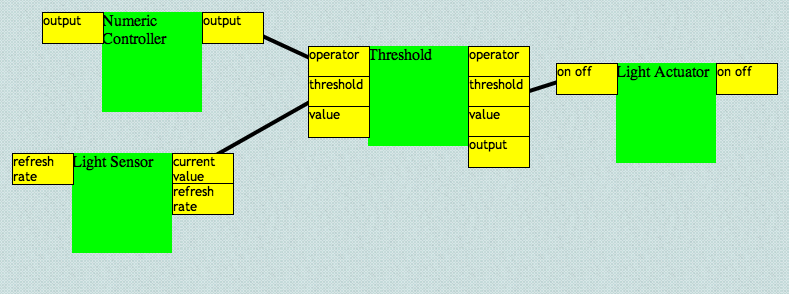
\includegraphics[width=\linewidth]{figures/fbp-application}
\label{fig:fbp-application}
\end{figure}

M2M applications are by definition distributed where the application
requirements involve a network of nodes collaborating for some common 
goals. M2M applications are typically defined by its flow of information
between components, as opposed to more traditional applications that focus more
on local information processing.

Flow Base Programming is best suited for describing M2M applications as it
allows the developers for the applications to focus more on the
abstraction meaning of the components instead letting the unimportant details
such as the hardware to stick right in the face. The result application will
contain all necessary information for the framework to construct low-level
details to implement the flow.

Applications are designed and constructed on FBP canvas by dragging a set of
abstract components from the library as illustrated in Figure~\ref{fig:fbp-application} 
Each component is
illustrated by a green block, each block has a set of properties, each with
different access modes, such as readonly, writeonly, readwrite. Properties on
the left of the greenblocks are properties that could be written, and
properties on the right are readable. Components are connected by links, which
is drawn by linking two properties in different components.

Some components represent physical hardware such as a sensor, or an actuator
while some other components could represent virtual processes such as
mathmatical computations, comparisons, etc. However, the final physical implementations
of the components are only made during application deployment by the Master but
not during FBP construction.

Components expose their interface through properties. A link is only made with
properties with matchinkg data type. The FBP applciation in
Figure~\ref{fig:fbp-application} illustrates a simple scenario where the light actuator
will turn on the light if light level drops below some value. The Numeric
Controller component will be assigned to a user input device used by users to
set its desire light threshold, which its output is sent to Threshold
component. The light value is sensed from Light Sensor component and sent to
Threshold. If the light value sensed is below the threshold value, Threshold
will output a boolean to set the on off property of Light Actuator to turn the
device, which will be deteremined during deployment, that it is represented by
on or off.

\subsection{Sensor Profile Framework}

While FBP defines the logical view of an application, WuKong profile framework allows
tracking, identification of physical resources within the Sensor Network.
There are a range of sensors which provide similar functionality with different
level of quality, it could model the sensor capability to enable handling
heterogeneous sensors and provide a common abstraction for the logical view.

There are two main concepts in Sensor Profile Framework, WuClasses and
WuObjects. WuClasss model components by exposing a number of properties
describing, and allow access to, a specific resource represented by the class.
Drawing from the example in Figure~\ref{fig:fbp-application}, the on off property of Light
Actuator component is boolean writeonly. WuClass also implements an update()
function to describe a component's behavior. For
example, Threshold has four properties: operator, threshold, value, output. The
output value is determined from the previous 3 properties that it returns true
when the value is lower or higher than the threshold which depends on the value
of the operator, and it returns false otherwise.


WuObjects are the main unit of processing that are hosted on the nodes. Each
WuObject is an instance of WuClasses. It allows the framework to achieve
4 responsibilities:
\begin{enumerate}
\item Allow the Master to discover the current status of a node with the list
of WuClasses and WuObjects it has.
\item Create new WuObject instances on a node to start receiving data and doing
local data processing.
\item Trigger executions in WuObjects, either periodically or as a result of
changing inputs.
\item Propagate changes of properties between linked properties in different
components, which may be hosted locally or remotely.
\end{enumerate}

\subsubsection{Property Propagation}

The profile framework is in charge of communication between WuObjects as
well, which are not necessarily on the same nodes. Profile Framework monitors
the changes in properties and propagate the changes to the connected WuObjects.
For example, if a Temperature WuObject is connected to a Threshold WuObject,
the changes in Temperature current value property will trigger propagation from
the Profile Framework to propagate the new value in current value to the
Threshold WuObject connected property, and since Threshold WuObject could be on
a different node, the framework will take care of this by initiating
a wireless connection between the nodes to send the data over. Once a new value
has been set, Threshold WuObject will also trigger its update() function to
recompute its output properties which in turn would cause another chain of
propagation to the linked WuObjects.

\subsection{Compilation and Mapping}

\begin{figure}[h!]
\caption{WuKong application build flow}
\centering
    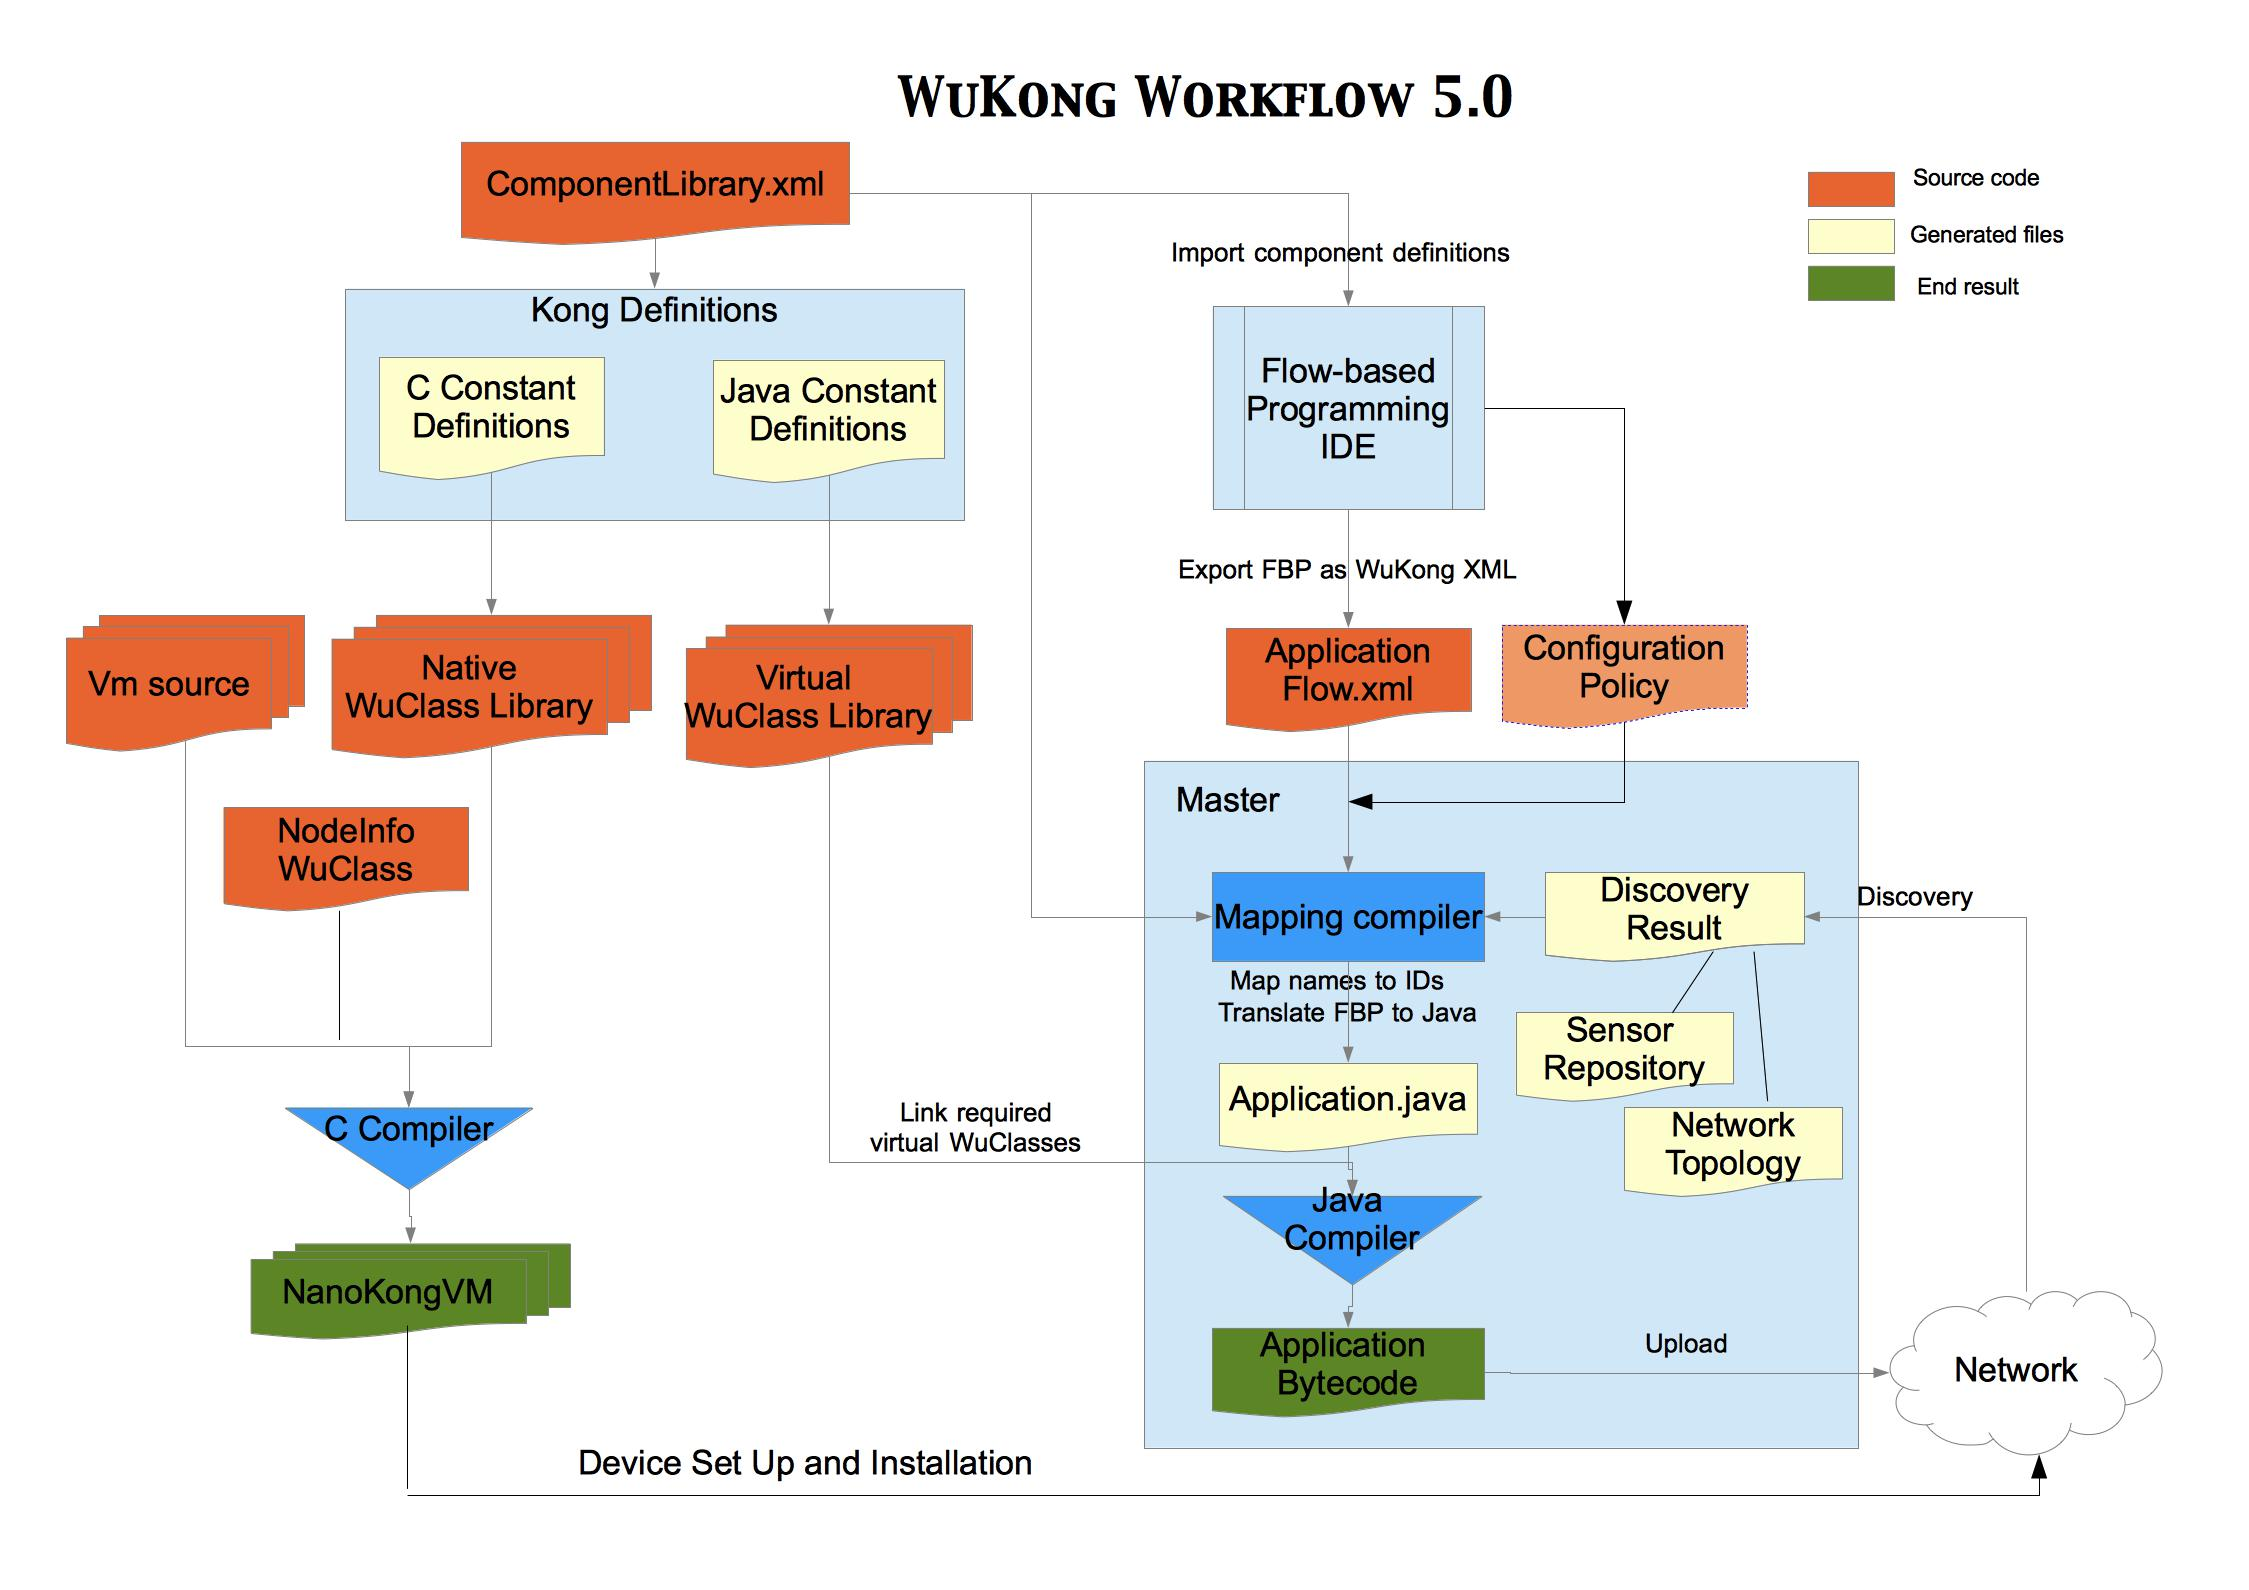
\includegraphics[width=\linewidth]{figures/wukong-flow}
\label{fig:wukong-flow}
\end{figure}

Figure~\ref{fig:wukong-flow} shows the overview of WuKong's build flow. The
left part represents the build process for NanoKong VM which will be installed
on the sensor nodes as part of the WuKong framework. The top part represents
the build process for generating component libraries and Virtual WuClass
library which will be used in other parts of the process. The right part
illustrates the build process for FBP applications from being drawn in the IDE
to Java bytecode that will be transmitted to the nodes.

The FBP program from the IDE will be exported as XML to the Master, the Master
will then take this XML and passed to Mapper to generate a Java program that
will be executed on the nodes. Finally, the compiled code is then wirelessly
uploaded to the nodes in the network.

The Java code consists of many parts from different phases of the mapping process.
First, the Java code contains information about links between components that
were taken from the FBP XML passed in earlier from the IDE. A link contains the
source component id, destination component id. The library code for components
corresponding to the component ids are stored in the node if it is written in
native language, or uploaded as part of the Java bytecode if it is written in
Java language. Second, it contains information about the mapping from
application component ids to actual node identifications and positions. The
purpose of a mapping which separates from the actual link makes it easier to
substitude the actual host of the WuObject later during
reconfiguration from the Master. This mapping is created by the Master during
discovery phase that probe the network for node's capabilities in terms of
available WuClasses, then mapper will decide the final candidates that will be
hosting for a component. If no native version of a component is found on the
nodes, mapper will substitute with a Java version of it.

\subsection{System Progression Framework}

There are a few popular wireless communication protocols in M2M applications:
ZigBee, ZWave. It is expected that in the future more diverse
wireless nodes equipped with radios that support protocols such as low-power
bluebooth and WiFi that all have one or more powerful gateway to connect to the
outside world. In WuKong system, one of the gateways will take on the role of
higher management decision maker called \emph{Master} to making the decisions for
deployment and producing the configuration of wireless sensor networks.

% TODO:probably need more here

\subsection{User Policy Framework}

\begin{figure}[h!]
\caption{A user component policy dialog}
\centering
    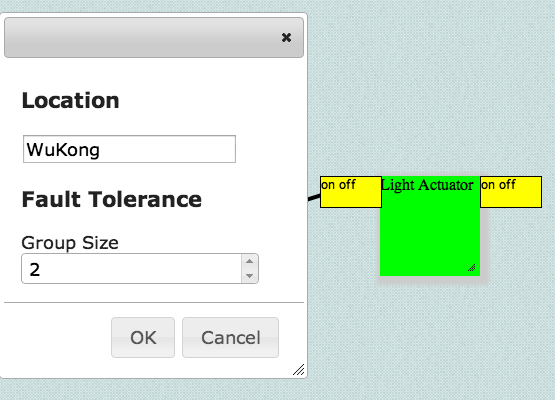
\includegraphics[width=\linewidth]{figures/fbp-policy}
\label{fig:fbp-policy}
\end{figure}

Many M2M applications are heavily influenced by user preferences and current
environmental context, as users and objects are mobile and application
requirements and policy could change in time. Users are able to specify
user policy for every component in the FBP and the application as a whole as
illustrated in Figure~\ref{fig:fbp-policy}

\subsubsection{Fault Tolerance policy}

M2M applications are inherently distributed, and hence it is inherently prone
to failures since all nodes are running autonomously unattended for a long
period of time where the external enviornmental influences could break and shut
down the devices easily. Fault Tolerance policy enables users to specify
relevent policy for tolerating failures in the granular level. This thesis will
discuss more on fault tolerance policy in the following chapter.

\chapter{Related Work}
\label{c:intro}

\section{Component Based Middleware}

Distributed Systems such as Wireless Sensor Netweorks (WSNs) composed of
multiple resource constrained devices equipped with low-power radios, low-cost
sensors collaborating to perform tasks for applications in multiple discipline
such as habitat monitoring. However, typically WSN applications are huge in
scale, subject to unreliable network, high risk of node failures, and expected
to run unattended for a long period of time, several work on lightweight component
models have been proposed\cite{Costa2007}\cite{Gay2003}\cite{Coulson2008}.

% About LooCI and REMORA
\subsection{Lightweight Component Models}

Work such as LooCI by Hughes et. al.\cite{Hughes2012} and Remora by Taherkordi
et. al.\cite{Taherkordi2010a} have demonstrated the feasibility of
reconfigurable infrastructure with event-driven programming model, event
management system, dynamic-binding to reduce development overhead, simplify
abstractions, and easier, dynamic reconfiguration for distributed applications.

\section{Fault Tolerance in Distributed Systems}

Many systems has been proposed to provide fault tolerance in distributed
systems, as the possibilities partial failures is a fundamental characterisics
of distributed systems.
However, distributed systems such as Wireless Sensor Networks typically
involves a large number of resource-constrained devices equipped with various
hardware components such as microprocessors, sensors, memory, wireless
communication. An application rely on the collaboration among the sensor nodes in
the network to perform tasks.

% No single point of failure

In order to prevent a single point of failure in applications that would bring
application to a halt in the event of failure, 
one of the primary goals for most of the work for fault tolerance is to
eliminiate single
point of failure in an application, so replications, redundancies are
recognized to be a good model for tackling the problems mentioned earlier in
distributed systems.
% replication and redundancy
Replication and redundancy are both techniques that allow the system to
duplicate multiple copies of a specific system component such that in the
event of failure of one of the components, one of the other duplicated
components can take over to perform the same services or functionality that the
previous one provides.

\subsection{Group Communication System}

Some work emphasizes on providing a set of group communication protocols to
ensure the information among a single replication or redundancy group could be
synchronized\cite{Sussman2000}. By modeling replications and redundancies into
a single system component unit in fault tolerant distributed applications, 
Sussman et. al. work on Virtual Synchrony could allow an efficient, distributed
way to manage replications autonomously.

\subsection{Multi-Agent System Resource Allocation}

Luna et. al.\cite{Luna2008} proposed a new approach to building reliable
Multi-Agent Systems involves assigning agents to machines to manage resources,
and by measuring the criticality of the components in real time to replicate
only for critical agents under system resource constraints for fault tolerance.

\subsection{Service-Oriented Architecture}

Neumann et. al.\cite{Neumann2010} proposed a new redundancy infrastructure to
bring Service-oriented Architecture (SOA) to Wireless Sensor Networks (WSN).

SOA is an established approach to ease development of complex distributed
applications by encapsulating system compoennts into services, this allows a more
flexible way to construct and develop interactions in application.

% what they lack for solving the problems I face
However, these approaches don't work well with applications where
reconfigurability, interoperability, and heterogeneity are requirements.
Existing approaches do not consider reconfigurability in the
application level that might invalidate existing infrastructure built upon one
instance of applications in another new instance when redeployed.
Most existing approaches also are not efficient in providing reducing the
development overhead to simplify fault tolerance in existing applications.

\chapter{Fur: An Intelligent Fault Tolerance System}
\label{c:fur}

This chapter describes how subsystems in Fur collaborate to provide fault tolerance
for applications. First we will describe how users could specify fault
tolerance policy for the application, and then how WuKong Master take
the policy, application and discovery results and compile into low-level
intermediate representation that could be deployed to the network. Lastly, we 
describe how the sensor network detect, recognize, and recover from failures
autonomously based on the result of the mapping.

\section{WuKong Applications}

~\ref{application} illustrates a typical WuKong application with components
connecting to form a small network. What this figure shows is that applications
are made of components, and components are connected through properties.
Any pair of properties form links that binds components together. Connected
components interact with each other based on the direction of the connection.
The properties on the left of a component are inputs to this component, to the
right side are the outputs of an component. Thus one can infer that
a connection cannot connect to both inputs or outputs of any pair of components
as both of them have the same data flow.

\section{Fault Tolerance Policy}

In this work, fault tolerance policy can only be specified on the level of
components, so there is a separate policy for every component. For every
compoennt, users can specify two rules to guide and influence how fault
tolerance works at the hardware level.

\begin{enumerate}
\item[Minimum Redundancy Level] The minimum number of devices that will be
supported as a backup for a particular component. Therefore when one of the
devices fail, others will take over.
\item[Maximum Reaction Time] The maximum latency a failure will take to detect
within the heartbeat group it is detected.
\end{enumerate}

The policy for every component will be taken by the WuKong Master, along with
the FBP application and discovery results, to produce the final mapped results
that could be compiled into low level bytecode that would be executed on the
network.

\section{Redundancy}

The primary design for fault tolerant distributed system is based on the
concept of redundancy and distributed systems usually have advantages to have
spare resources. Not only it is good to combat partial failures, it also
provide durability to the system for an extended period of time.

Spare resources address the first fundanmental characteristics of fault
tolerance that there is no single point of failure within the system.

One of the challeneges in producing a fault tolerant design in a heterogeneous
network modeled by the WuKong's sensor profile framework is that devices are
partially homogeneous, meaning that the hardware setup is different from node
to node, so it is not straightforward to simply assign a device as a complete
backup of another device.

The solution introduces two new system abstractions that could address the
challenge: Recovery chains and heartbeat groups.

\section{Mapping for a fault tolerant system}

The figure~\ref{} above illustrates the essential parts in the mapping process
for a fault tolerant system.

Mapping is a process of converting a high level abstractions from FBP with
components to low level bytecode representation that will be deployed to the
network.

Heartbeat is an important mechanism to detect failure. Our work assume
a fail-stop model where sensor nodes fail by not sending messages for a period
of time. Mapper will have to determine the heartbeat arrangement, dependencies
to ensure every sensor node is monitored and will not fail without notice.

\subsection{Heartbeat Group}

Heartbeat arrangement usually depends on the applications and sensor
arrangement~\ref{}, thus most related work aim for a specific type of
application and sensor arrangement to simplify heartbeat arrangement, however
since application type and sensor arrangement in WuKong are not known until
deployment, therefore a new way to arrange heartbeat has to be devised.

In WuKong, application are drawn on a canvas which consists of blocks that
gives the type of sensors or resources needed and lines which connects the
resources together in such a way that would satisfy the requirements. However,
arranage heartbeat based on the flow of the components is not desirable since
applications are not the immediate representation of the underlying network
topology such that some components could be mapped on the same node, and some
connected components could be mapped to nodes that are far away from each other
that require multiple hops to reach. Arrangement based on such high
abstractions would incur extra communication overhead by making a lot of nodes
as a relay for heartbeats.

The proposed solution will produce application agnostic arrangement and at
the same time be used in producing the arrangement of the compoennts in the
network to reduce the communication overhead as much as possible.

Assuming that links are symmetrical and toplogy is stable after making the
arrangement, we proposes the algorithm below to produce heartbeat arrangement
for applications.

\begin{algorithm}
\caption{Determine Heartbeat Arrangement}
\label{alg:heartbeat-group}
\begin{algorithmic}
\Require A list $N$ of node ids of the network
\Require A function isNeighbor that returns a boolean for whether a pair of
  node ids are neighbor
\Ensure A list of lists $H$ which contains the node ids of the groups
\While{$|N| > 0$}
  \State Pick a random $i \in N$ as anchor node
  \State Create a new list $h$
  \State Add $i$ to $h$
  \State Remove $i$ from $N$
  \For{Every $n$ in $N$}
    \If{isNeighbor$(i, n)$}
      \State Add $n$ to $h$
      \State Remove $n$ from $N$
    \EndIf
  \EndFor
  \State Append list $h$ to $H$
\EndWhile
\end{algorithmic}
\end{algorithm}

The algorithm~\ref{alg:heartbeat-group} will produces a clustering with nodes
that are one hop distance to each other, in other words, fully connected. By
grouping nodes within one hop distance together, we significantly reduce the
possibility of heartbeat hopping which is a big factor in communication
overhead.

The implementation of the function isNeighbor depends on the actual hardware
used, if it is using ZWave, then it will query ZWave for information.

The worst-case time complexity of the algorithm is $O(n^2)$ given a list of
disconnected nodes since every single one will form a group of its own,
therefore the inner loop will be running for every node in the list, thus it is
quadratic.

The best-case time complexity is $O(n)$ when the nodes are fully
connected, since the inner loop will be executed only once.
% possible need some more explanation here :\

The it is possible that due to some peculiar network topology that the
algorithm would produce single node group which itself could not be of any use.

If that happens, the algorithm will be rerun again. Since the anchor is picked
randomly from the remaining node list, the algorithm will not produce the same
result thus eliminating the problem.

\subsection{Recovery chains}

When a component FT policy indicates a minimum redundancy level higher than
one, WuKong Master will map multiple eligible nodes to carry the WuObject
coresponding to the component and become the backups in case of a failure.

Since nodes could carry more than one component WuObject, and we assume
a heterogeneous network where it consists of nodes with different combinations
of capabilities, so for every comoponent WuObject there should be an ordered
list of nodes like a chain of command that when one of them failed, the next
one will be able to replace its place.

When a failure is detected, the detector is not necessarily carrying or knowing
what resources there are in the network at the given moment, and it would
produce an enormous of overhead to query for the resources in the network, so
with this ordered list of recovery, the information could be stored in advance
to prevent nodes having to do all the work over and over again whenever
a failure is detected. 

After mapping, the information of recovery is distributed accordingly based on
the heartbeat group results to ensure the integrity of recovery process such
that the detector will be able to recover broken links and update the nodes
that are affected.

The algorithm to produce the recovery chains is shown below, and it is
separated into several sections.

\subsubsection{Gather Candidates}

First it would have to sort and filter from the list of nodes discovered, which
are eligible to provide certain resources for components specified in the
application. Once it is sorted out, the algorithm will produce a dictionary of
component id as keys and list of node ids as values.

The algorithm requires node info of each node in the network. A node info
constitudes information such as a list of WuClasses and a list of WuObjects
that are used to help Master greatly in making an informed decision to gather
a list of eligible candidates for components.

\begin{algorithm}
\caption{Gather Eligible Candidates for Components}
\label{alg:recovery-chain}
\begin{algorithmic}
\Require A list $C$ of application component ids
\Require A list $I$ of node ids of the network
\Ensure A dictionary $D$ of component id as keys and list of node ids as values
\Function{isCapable}{$i, c$}
  \If{ComponentToWuClass($c$) in WuClasses($i$)}
    \State \Return \texttt{True}
  \Else
    \State \Return \texttt{False}
  \EndIf
\EndFunction
\For{Every $c$ in $C$}
  \For{Every $i$ in $I$}
    \If{isCapable($i$, $c$)}
      \State Add $i$ to $D$ under component id $c$ as key
    \EndIf
  \EndFor
\EndFor
\end{algorithmic}
\end{algorithm}

Function isCapable returns a boolean for whether the node is capable of
carrying the component

This algorithm will filter out and produce a list of eligible candidates for
every application component.

\subsubsection{Redundancy Level Enforcement}

Once the candidates has been gathered for every compoennt, here it will be
doing a check to enforce redundancy level policy to make sure all gathered
candidates are above the minimum redundancy level. If any of the candidates is
not satisfied, the deployment process will be terminated and the system will
send a warning to the users to inform of this situation.

\subsubsection{Sort Candidates}

It would be perfectly safe to deploy at this point with the unsorted candidates
for each component, but it will be running into a problem that could compromise
the operation of the system by unoptimized component arrangement. If the
components placement is unsorted, it is possible that unnecessary communication
would saturate the system thus compromising the health of the application. On
the other hand, if the placement is carefully analyzed, the impact of the
overhead could be minimized to certain degrees such that the system could run
when deployed.

\begin{algorithm}
\caption{Build histogram of the nodes appear in candidate list}
\label{alg:build-histogram}
\begin{algorithmic}
\Require A dictionary $D$ of unsorted recovery chains of every component
\Ensure A dictionary $H$ of node ids and number of occurrances
\For{Every $c$ in $C$}
  \For{Every $n$ in $D[c]$}
    \If{$n$ not in $H$}
      \State $H[n] = 1$
    \Else
      \State $H[n] = H[n] + 1$
    \EndIf
  \EndFor
\EndFor
\end{algorithmic}
\end{algorithm}

\begin{algorithm}
\caption{Sort Recovery chains}
\label{alg:sort-recovery-chain}
\begin{algorithmic}
\Require A list $C$ of components
\Require A dictionary $D$ of unsorted recovery chains of every component
\Require A histogram $H$ of all nodes
\Ensure A dictionary $D$ of sorted recovery chains of every component
\For{Every $c$ in $C$}
  \State Sort $D[c]$, and use $H$ as keys in decending order
\EndFor
\end{algorithmic}
\end{algorithm}

By sorting based on the occurrances of node as candidates, the nodes with
highest scores will be hosting a lot more components thus reducing external
communications within the system especially for the case when WuObjects are
linked but are placed in separate nodes.

\subsection{Determine Heartbeat Group Period}

Once the placement and ordering for the components in forms of recover chains
are decided, the heartbeat interval for heartbeat groups could be deteremined.
Since heartbeat groups could have multiple components, the group heartbeat
period is half of the minimum maximum reaction time policy of the components.

Our system assumes a fail-stop model where nodes are suspected dead when it
does not send out messages, but to compensate possible deviation in
communication latency, a failure is detected when the node does not send
a heartbeat message within two normal heartbeat periods. Thus the heartbeat
period is half of the reaction time.

\begin{algorithm}
\caption{Determine Group Heartbeat Period}
\label{alg:determine-group-heartbeat-period}
\begin{algorithmic}
\Require A list of heartbeat groups $H$
\Ensure A list of heartbeat groups with heartbeat periods
\For{Every heartbeat group $g$ in $H$}
  \For{Every component Component($n$ in $g$)}
    \State Find the lowest minimum reaction time
    \State Divided in hald and assign the period to group $g$
  \EndFor
\EndFor
\end{algorithmic}
\end{algorithm}

Since all nodes within the heartbeat group is compared against, so only the
lowest time will be picked.

\section{Information Distribution}

After mapping and produced heartbeat groups for the network and recovery chains
for the components, WuKong would have to generate and assignment information
appropriated to every node to support fault tolerance.

Every node will have information pertain to the list below:

\begin{enumerate}
\item Recovery chains for the mapped components
\item List of nodes of the heartbeat group it is in
\item The recovery chains of the node it will monitor based on
the heartbeat arrangement
\item The application links of the components assigned to the node it will
monitor based on the heartbeat arrangement
\item Heartbeat period of the group it is in
\end{enumerate}

\section{Application generation}

WuKong runs a JVM on every node in the network, the VM provides services for
the application program in Java to access lower parts of the resources.
This section will introduce the list of newly added interfaces and resources to
support and enable fault tolerance for the application.

\begin{enumerate}
\item component instance id to WuObject address map
\item heartbeat groups member list
\item heartbeat group period list
\end{enumerate}

\section{Wireless Deployment}

The rest of the deployment is the same as the deployment described in the
background work for WuKong, where after it generates the Java code, it compiles
down to lower bytecode representation and send it to every node wirelessly. The
nodes will be reprogrammed by taking the code and reload in their flash memory.

\begin{comment}
\section{Questions}

Q: How does the system recover from two consequtive failures in the network?

A: We assume a much simpler failure model where there can be at most one
failure happen at any point in time. It is a reasonable assumption given that
our system recover from failures fairly quickly (~2 secs) ....


Q: How does an application is being compiled into low level bytecode? And when
and how does WuKong reconfigure the nodes?


Q: What happen when an application is deployed? What is specifially at work?
\end{comment}

\section{Fault Tolerance System}

\subsection{Member ranking}

% transition to failure diagnosis, and failure recovery, and member ranking
If application could specify a full ranking among a group, 
Whenever a leader died, a member has to replace its position.
Leader identification, successor of current leader.

 agent should specify whether this group has any ranking rules for a members. Whether there is a full ranking for current members and future members. This could lead to different actions reacting to similar events. ...

\section{Agent architecture}

This section will first go into details of how applications in a form of an
abstract graph are being managed in a distributed system after being compiled 
and transformed into lower bytecode representation, then I will further discuss 
how the agent architecture on every node collaborate to form groups that will 
be the basic unit of redundancy in the application to detect sensor failures, 
diagnosis the failure, and finally recover from failure.

~\ref{} illustrates the proposed agent architecture in the sensor network.
Every component in the application is converted into groups, which consists one
or more nodes, and one of them is a leader. Every group has only one leader.
Heartbeats are sent out from the members and leaders to monitor each other.

\subsection{Autonomous Systems}

Sensor networks composed of a large number of diverse subsystems. Subsystems
intertwined with complex relationships that prohibit human intervention.
Subsystems such as deployment, operation, reconfiguration, maintenance must be
automated.

The inability, passiveness to errors makes the past systems unable to deal with
perturbations, or unpredictable changes in the environment. Such systems know
a limited amount of patterns and trigger predefined actions when they encounter
these patterns. In order to make system adapt to new environment in a way
similar to biological systems, they need to react to events as a whole in
real-time.

\subsection{Distributed agents}

As our system consists of complex elements and subsystems mingled together, an
appropriate way to handle complex behaviors in decentralized systems is to
based it on a society of agents.~\cite{Minar1999}

\subsection{Towards failure detection}

As we mentioned earlier why sensor systems has to evolve to adapt to crutial,
ever changing environment, one of the first things a system could achieve that
goal is to detect failures autonomously.

\subsubsection{Group membership}

In our model, sensor networks consists of a diverse of sensor platforms, and some
subset of sensor nodes are equipped with similar sensors situated near each other.

Since sensor networks are inheritly concurrent, it is very hard to reason about
the states of the nodes in a distributed fashion. In order to provide fault
tolerance in the system, a number of nodes need to be in sync and form a group
to monitor and replace faulty node if necessary.

~\ref{} illustrates a running applications with three components: Temperature,
Light and Threshold. Every component is implemented by a group of sensors
hosting the same object that represents the component.

Every node consists of two agents, namely membership and controller as
illustrated in the~\ref{}. When application is deployed, every node is populated with a link table full of links and a list of objects representing the components on the application that are being assigned to.

Membership agent is there to maintain and update the membership list by
also managing a watchlist and a reportlist to receive/send heartbeat from/to.

\paragraph{Heartbeat and node failure}

% what is a failure, why we assume fail-stop failures

A failure in distributed system could come from different sources. Some nodes
might fail because of software bugs; some nodes might fail because of poor
wireless link quality caused by interference. One of the biggest challenges in
distributed systems is to be able to detect the types of failures when it
occurs correctly. Pulled between efficiency and reliability, decisions to make
individual sensor nodes at the same time able to detect failures with knowledge
of others but also have to reduce the amount of resources is essential for
designing a effective distributed system.

% Brief introduction to Byzentine failures

There is another type of failures caused by a completely different reasons.
Byzentine failures are failures inspired by the Byzentine General's Problem
where components of a system fail in arbitrary ways (besides stopping or
crashing) by processing requests incorrectly, corrupting local states, or
producing incorrect or inconsistent outputs.

% Why we choose fail-stop failures

As we assume society of cooperative agents, every agent in the system will
strive to be helpful, and share a common goal. This is strengthen by the fact
that the agent goals' are bootstrapped from a common source which is the WuKong
Master. However, nodes could still fail. In order to be consistent, we model
failure by whether a node could send messages or not. This is called
a fail-stop failure model.

% What we choose

A fail-stop failure model is a model in which sensor nodes are suspected of
failure when they stop sending messages which could caused by multitude of
reasons such as network partition, or software bugs.

% what is a heartbeat

Heartbeats are messages sent by individual nodes periodically to indicate to
the monitoring nodes its health~\cite{}.

~\ref{} illustrates some nodes sending heartbeats that detects
a failure when a number of expected consecutive heartbeats have not been
received.

% what is a failure in our model

A node is considered dead when it has not been sending heartbeats for more 
than 2 rounds of timeout.

\paragraph{Group setup}

The WuKong Master has already assigned an ordered list of nodes for every component,
every node would be able to know who are in their group for any particular
component.

Wielded with this knowledge, membership agent will setup all heartbeat links
between the nodes if not already.

Since the setup is asynchronous without lockstep, all nodes are free to do
whatever they want while others are being programmed. We added a random backoff
after the nodes are programmed to prevent the problem of nodes reporting 
failure when they startup, because when the node finished setup, the nodes it
is watching might not be finished reprogramming, thus it will delay its
heartbeat and exceed the timeout causing the node to send false alarm.

As illustrated by~\ref{}, every node has a leader which is elected when the
group is formed.

\begin{figure}[h!]
\caption{Node states}
\centering
    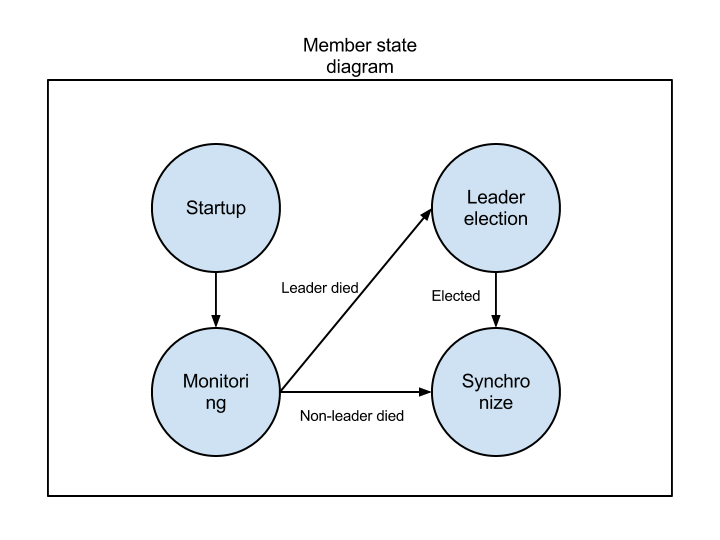
\includegraphics[width=\linewidth]{figures/node-states}
\end{figure}

\subsubsection{Connecting them up}

% what happened when a node fails?

When a node failed, or has not sent heartbeats for too long, a node failure
will be picked up by the monitoring nodes. However, a system is not fault
tolerant if it cannot decide who could be replacing the failing component. So
there must be some way to organize groups such that when a failure is detected,
a replacement could be decided.

% introduction to heartbeat network

It is possible that there will be multiple failures occurred in a timely
fashion. We need to be able to detect all possible failures within a group, so we need a heartbeat network.

% talk more about heartbeat network

Of course the structure of heartbeat communication pattern highly depends on the underlying network assumption and infrastructure of the application. To produce the most efficient network with the least connections, heartbeat network has to satisfy two properties.

\begin{enumerate}
\item Every node has to monitor at least one node other than itself
\item Every node can only has one node monitoring itself
\end{enumerate}

% why daisy chain, what's the benefits? How does it affect other fault
% tolerance policies?

A heartbeat network in the form of a daisy chain is one of the networks that
satisfy both properties as shown in~\ref{fig:daisy-chain}. Every daisy chain heartbeat network monitors all nodes
in the group, given by the properties that every node has to monitor at least
one node and every node can only have one node monitor itself. So if there is
n nodes, there can be at most n nodes being monitored, every monitoring node
can only monitor one node, every node can only monitor node that others have
not, thus every node is monitored by only one unique node. Thus this daisy
chain guarantees every failure can be detected.

\begin{figure}[h!]
\label{fig:daisy-chain}
\caption{Daisy Chain of heartbeats}
\centering
    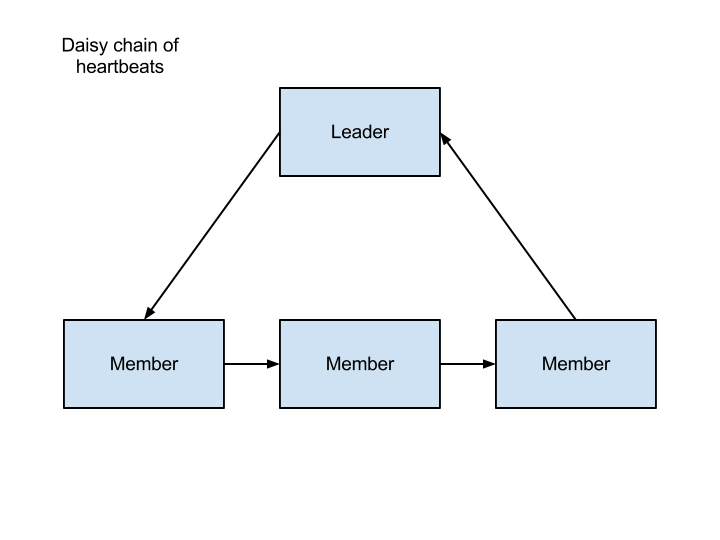
\includegraphics[width=\linewidth]{figures/daisy-chain}
\end{figure}

%\subsubsection{Multi-component nodes}

%Each node maintains a watch list of nodes that it has to monitor health for. The watch list is generated by iterating through all groups and one node from each group that it has to monitor. The watch list is a set, so there will be no duplicate entries, every entry is unique in the watch list.

\paragraph{Message complexity}

Every heartbeat takes one message to send from one to another. As of current,
      we assume every heartbeat is sent using unicast, and there is no ACK for
      heartbeat messages. The message complexity for standard one-hop star
      network takes about
      O(2n-2) messages since the leader sends n-1 to every member and every
      member would also has to send a message back to leader, that comes to
      double of the single traversal from leader to other members.

The message complexity for the daisy loop takes about O(n) messages for a group, because every member only sends one heartbeat to one other member at a time including the leader.

\subsection{Failure recovery}

% mention the needs for at least one substitude, and how the candidate is
% selected

When a node failed, it is guaranteed that at least one node will detect
this. However, the chain is broken, and it would be impossible for the
membership agent in the node to decide what the subsequent actions could be.
They are not designed to do such things.
There need to have another agent to decide based on local information the
actions to take to resolve this issue.

\subsubsection{Link table entry protocol}

% What is link table

When the application is deployed, every operating node contains at least one
object that represents one component in the application. To connect the objects
just like what it did in the application as shown in FBP needs a table to store
the information of the links. Link table is broken down into two layers, where
the top layer gives the information between two components, and the bottom
layer gives a list of nodes that are part of the same group that could provide
the service for operating the application. By breaking into two layers gives
us immense flexibility to handle many different kinds of graph that the FBP could
produce.

% Why a protocol for link table

As illustrated in~\ref{link-table-switch}, the premise of a link between
components rely on both end's agreement. If either one of them disagree, then
the link is not valid.

When a leader of a component failed, the elected new leader will have to update
everyone’s
link table so they all are in consensus of who is currently the representative
for this component. The result of the protocol affects the lower layer of the
link table, so all nodes in the network affiliated with a particular component
could be assure that they are not sending messages to nodes that doesn't exist 
or listening for messages from nodes that are not in charge of sending the
sensor values.

\begin{figure}[h!]
\label{link-table-switch}
\caption{Link table switching}
\centering
    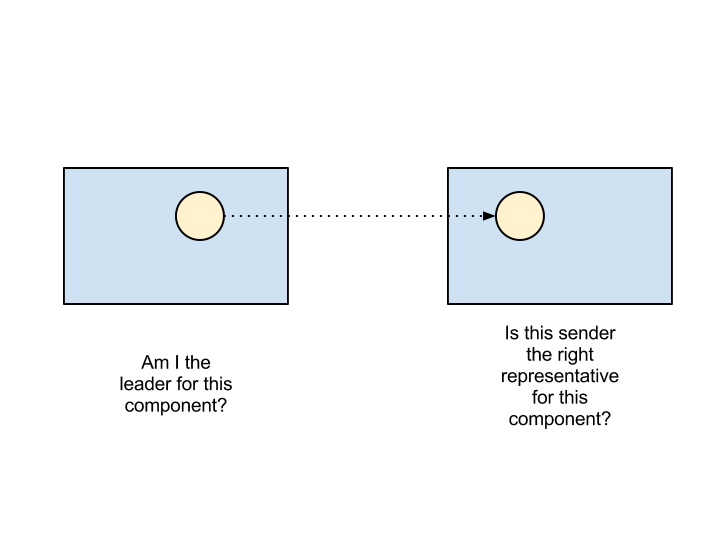
\includegraphics[width=\linewidth]{figures/link-table-switch}
\end{figure}


\subsubsection{Controller agent}

We have described a part of the system that does membership, fault detection.
However with only those parts the system, they do not form a fault tolerant
system. Without a controller making a right decision at the right time,
to synchronize group states, groups will not have consensus and will not be
able to proceed as a whole~\ref{}. Controller’s responsibilities range from
responding to
failure events, synchronizing states to group members and connected nodes to 
ensure the application could still operate.

Reactions and actions tables are set up during deployment. Controller will be
mainly handling events and handle according to the rules defined in the
tables.

\paragraph{Member ranking}

Most other work on failure recovery relies on leader election to elect a new
leader when the old leader failed which is followed by a group multicast to
ensure group state is synchronized to all members.

However, leader election is not necessary if a full member ranking could be
determined. Member ranking serves as a lookup table to successor to any node if it
happens to fail, also used to recover heartbeat network.

%TODO: expend this and explain a bit more with figure and examples

\paragraph{Responding to failure}

~\ref{} describes the dynamics between agents when a failure has been detected.

When a member detected a failure from other member, the membership agent on the
member node will notify local controller agent of this event. 

By default, controller agent will notify the leader of the group if it is not,
the leader’s controller agent will initiate synchronization protocol to
synchronize members’ membership list.

If the leader failed, the controller agent of the monitoring node will initiate
the leader election protocol and become a new leader itself.


\paragraph{Leader election}

% Explain why we need leader election
When there is no clear ranking among members, a leader election could provide a mechanism for determine the successor of a failed node.

% But explain about how member ranking could be used to eliminate leader election

% Then explain that heartbeat network is used as an indication of ranking
% between members



% Need a new figure for leader election with member ranking
%\begin{figure}[h!]
%\caption{Leader election diagram}
%\centering
    %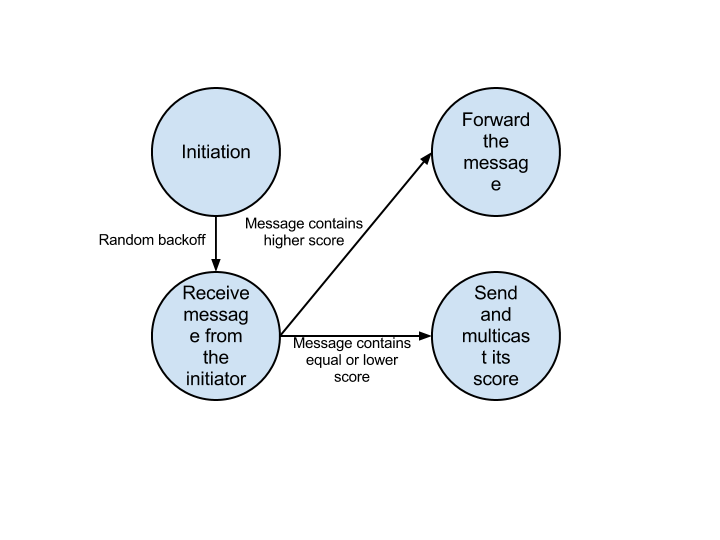
\includegraphics[width=\linewidth]{figures/leader-election-1}
%\end{figure}

\paragraph{Recover from failure}

% confirm and update local membership table


% synchronize membership table in group

\emph{Membership synchronization}

Some actions will be syncing membership list across all members for a particular group. This protocol is triggered either by the reaction table above or by explicit request from other agents, such as the Membership agent. Controller agent will access the current membership table and instruct Synchronization agent to start the membership list synchronization.

% synchronize link table in group and connected nodes

\emph{Link table synchronization}

Once the fault has been confirmed and has shunned the faulty node from the network, GMS coordinator will be responsible for propagating this event to other groups in the system that has subscribe to this event.

Let's say that a group has a simple one hop star topology, so all nodes will transmit its data to the group leader, when the group leader has been reported to be partitioned away from the network or failed, then what will happen is that each group member will elect a new leader by some heuristics, since it has the link table for the previous group leader, it will know which node it is suppose to link to outside the group upstream, and change its local link table accordingly, the new leader will determine the new linking table of its members by consulting the group policy, send a multicast to the group to route all their data to the new leader. The upstream node should either be inside a group managed by the GMS, or a Master assigned gateway, it should also receive this update according to the group policy which GMS will also inform them of.

Essentially, GMS is global in the network and will have full knowledge of the group policy for all groups in the application, and it can follow the group policy to propagation fault events to the appropriate groups.


\subsubsection{False positive fault detection}

It appears to be possible to have false positive fault detection when a node is not dead but actually got partitioned away from the network for a short period of time. If it is the leader that got partitioned away for too long, several members will be detecting this failure and they might all initiate a leader election. Since they all know of this situation, every node detecting a failure will wait for a random amount of time before sending the message. If a leader election message has been received, it will terminate its current action and continue to the second phase of the leader election process.

However, it is possible that leader is not actually dead, and it is also monitoring the members. The leader might conclude that the members are all gone and will also generate a failure event (since there is no one to synchronize to). This is a split brain problem because the remaining members will elect a new leader and proceed in synchronizing the link table in neighbor nodes, but the old leader is still operating and sending data between the neighbor nodes, this will create a conflict both in the group and cause a confusion among the outsiders.

Assuming both partitions can talk to the neighbor nodes with objects connected to their objects, there is no way for the partitions to detect the problem within themselves but only the outsiders.

The outsiders, whose objects are connected to the group, will be the fault detector and will notify both leaders of their existence along with their scoring. The leader with less scoring will give up their leadership, and try to merge with the other partition if possible. If it is still not possible after a timeout, it will try to notify the Master of this situation.

\emph{Daisy chaining}

Since it is also possible that heartbeat is in daisy chain that the any node only monitors one node at a time, and no two nodes monitor the same node. When that happens it is still possible that leader could partition away from the system and appear again later in time. Since the new leader is the one monitoring the old leader, when the old leader resume and start sending heartbeat, the new leader could be sending a reconfiguration message to Master, or if it is not severe enough to do a full reconfiguration, it could resign by sending the old leader a resign message to inform the leader to reconfigure its connected objects about this change of leadership, and it will resume to become a normal member again.

The message complexity for the operation of resignation should be O(2+2H(m)) where H is a function that returns the number of nodes hosting connected objects m.

\chapter{Experimental Design and Result}
\label{c:experiments}

\section{Experimental Setup}

\subsection{Sensor Nodes}

\subsection{Fault Tolerant Policy for FBP}

\cleardoublepage
\singlespacing
\chapter{CONCLUSION}
\label{c:conclusion}
\doublespacing\nointerlineskip

%Previous chapters have described the work that has been done on WuKong platform.
%It is useful to reflect on what has been accomplished and place them in the
%broader context of the more general fault tolerance problem as well as the
%specific contributions of this work.

\section{Discussion}

This thesis proposed a novel algorithm to achieve
recovery from failures by combining heartbeat protocol, for failure detection,
with Strips, which are used to maintain and track service redundancy.

We have presented a fault tolerance system able to provide failover for failed
services in service-oriented WSNs that comply with user policy requirements. We
have also described strip, a redundancy abstraction for service peers along with
distributed algorithms to synchronize strip views among members and
reconfigurate the network for the new structure to recover from node failure.
The system allows user intervention through means of user policy, which could
directly influence underlying system configurations and structure.

The developed methods add new and useful solutions to build a fault tolerant
system that could be reasoned easily and with a performance as expected on
average. This method makes an extension to other methods in terms of
completeness and complexity. It serves as a quick and easy solution
to provide practical fault tolerance for WuKong applications.

% TODO: summarize the results of the experiments here, etc
% e.g. The solutions developed for WuKong system performs very consistently, as
% the recovery time is always under two secs on average with a handful of
% sensors. However, occationally heartbeats could report erroneous failures and
% result in a quick false recovery, and left the partitioned nodes behind, but
% the system as a whole still function properly.

The experimental results have shown to be consistent and stable among first
failures in different rank of members in strip around 2.5 secs. The failover
have been successful in all deployments. It is also shown that the performance
degraded quickly when the hardware or the wireless communication quality
degraded. Therefore it is important that the network setup is as optimized as
possible. 

\section{Future Work}

% Probably move it to future work? Probably don't do it.
%Of course there are a lot of room for improvements. For example, if we want to
%go beyond this limitation of 232 nodes by Zwave, one of the ways we could do is
%to build another zwave network and have a routing agent to route messages
%between networks. And we would also want to handle network partitions. One of
%the possible research directions is to merge the partitions back to one if they
%come back together, or by using some arbitrary flags to indicate primary
%components in the network to eliminate redundant commanding network components.
%Nonetheless, it is also an opportunity to look into multi-hop networks since
%heartbeats protocols are designed with single-hop network in mind, whether we
%could change the protocol to handle multi-hop is also a big challenge a future
%research could take on.


We have shown a design for a reconfigurable fault tolerant system for WuKong.
Strips makes it really easy to describe a component system with redundancy for
heterogeneous services and devices. Nevertheless, there is still room for
improvements. This section will address some directions future research can take.

WuKong Fault Tolerance System did not consider for network partition. Network
partition occurs when a network of nodes got partitioned into two subnetworks where
none can detect each other for a period of time. One of the possible direction
is to create a more sophisticated failure model that could handle network partition.
In this thesis we assume failstop model where nodes, once dead, will not come
back. Therefore when network partition occurs, each part of the network would
not be able to recognize each other and would cause conflicts and confusions.

Our current heartbeat protocol is distributed and easy to construct, but it is
not shown to work under networks where messages are sent in multiple hops, since
the algorithm used to produce where each node should be sending heartbeat
messages does not consider the topology of the network. Heartbeat is sensitive
on latency, so if a heartbeat message was not received within tolerance period,
a failure event could occur and the node is suspected of failure and will
never come back. If the node is still alive, it would be treated as if it is
dead. And that will creates an artificial network isolation where a few nodes
are excluded from the network before of latency.

Current system can only allow the detector to handle one failure at a time. It
would be a desirable future research direction to investigate handling
consecutive node failures. One possible way is by storing ahead multiple nodes'
strips and heartbeat protocol data, such that when consecutive nodes failure
occurred the detector would be able to recover those services it backed up.
However there is a tradeoff on the memory a node could store and the number of
consecutive node failures a network could handle.

\begin{comment}
Niels suggested that I show that I am aware of such issue with determining
optimality for deployment which is not clear for WuKong yet, there are many
ways or metrics to optimize for, all I can do in this work is to identify some
tradeoffs certain deployment for fault tolerance could influence the system
with certain metrics.

Limits will be hard to define here
Niels:about the tradeoffs in determining the deployment from your fault
tolerance perspective
Penn:Remember what the prof told me, about policy, first fit, last fit, etc
\end{comment}

The optimization problem for application deployment is also an important element
in this system. This thesis didn't consider finding a optimal deployment for the
level of redundancy specified in the user policy. The problem of deploying
a specific distributed system onto a network structure typically consists of
mapping the components of the system onto the hosts of the network. The mapping
is subject to constraints. The constraints could be whether a node supports
certain service to host certain components, and how much communication overhead
would induce from the assignment to maintain consistency for the strips, and
from the perspective of WuKong, some components need to seaparate from other
components to achieve fault tolerance, and some needs to place together to
function properly.  Determining such an optimal deployment is a combinatorial
optimization problem, and combinatorial optimization problems generally
extremely challenging computationally. It is difficult to predict what will and
what will not work.  It is unlikely that a single approach will be effective on
all problems or instances of the same problems. As we also want the system to
come up with a solution within a time limit. So finding a good balance between
the quality of a solution of the time it takes to come up with a good enough
solution is critical.


\backmatter

\addcontentsline{toc}{chapter}{\bibname}
\bibliographystyle{abbrv}

% input your reference here
%\bibliography{thesis}
\bibliography{/Users/penn/Documents/Bibtex/Thesis.bib}

\appendix

\end{document}
